\chapter{Dependency grammar (DG)}
\label{ch:dependency-grammar}

The Stanford dependency analysis of a given text constitutes the input for the algorithm developed in the current work. It provides the foundation to build the syntactic backbone used adopted here. This chapter offers an overview of the grammar and the parser developed at the Stanford university. In the last part of the chapter is discussed the cross theoretical connection between the dependency and systemic functional grammars. 

\section{Origins of the dependency theory}
\label{sec:origins}
%In this section I outline the theory of dependency grammar. I will make references sometimes to concepts in SFG. 
For the first time a complete linguistic theory based on the dependency concept was elaborated by the French linguist Lucien Tesniere in his seminal work \textit{``Elements de syntaxe strusturale''} published in \citeyear{Tesniere59} after his death. He devoted much effort to argue for the adequacy of \textit{dependency} as the organizational principle underlying numerous phenomena and in fact attempting to demonstrate the universality of his syntactic analysis method for human languages. In doing so he introduced a series of concepts and ideas among which the \textit{verb centrality}, \textit{stratification}, \textit{language typology}, \textit{nuclei}, \textit{valency}, \textit{metataxis}, \textit{junction} and \textit{transfer} are the most important ones which I introduce following the connections.

%His work, originally in French, has been translated in multiple languages German, Russina, Spanish, Japanese, Italian and recently in English \citep{Tesniere2015}.

\begin{quotation}
    The sentence is an \textit{organized set}, the constituent elements of which are the words. Each word in a sentence is not isolated as it is in the dictionary. The mind perceives \textit{connections} between a word and its neighbours. The totality of these connections forms the scaffold of the sentence. These connections are not indicated by anything. But it is absolutely crucial that they be perceived by the mind; without them the sentence would not be intelligible \citep[3]{Tesniere2015}.
\end{quotation}

Tesniere holds the view that the connection, what is know today as \textit{dependencies}, are the foundations of the \textit{structural syntax} known as \textit{dependency grammar} today. According to him ``to construct a sentence is to breathe life into an amorphous mass of words, establishing a set of connections between them. Conversely, understanding a sentence involves seizing upon the set of connections that unite the various words'' \citep[4]{Tesniere2015}. He introduces the hierarchy of connections as follows. 

\begin{quotation}
    Structural connections establish \textit{dependency} relations between words. In principle, each connection unites a superior term and an inferior term. The superior term is called the \textit{governor}, and the inferior term the \textit{subordinate}. We say that the subordinate depends on the governor and that the governor governs the subordinate. [\dots] A word can be both subordinate to a superior word and governor of an inferior word. [\dots] The set of words of a sentence constitutes a veritable \textit{hierarchy} \citep[5--6]{Tesniere2015}.
\end{quotation}

Introduction of hierarchy and governor-subordinate dependencies permeates to define now what is a \textit{node} and the \textit{stemma} resembling what is now known as \textit{dependency tree} (although the stemmas do not include labels on the tree edges). 

\begin{quotation}
    [\dots] In principle, a subordinate can only depend on a sole governor. A governor, in contrast, can govern multiple subordinates [\dots] Every governor that governs one or more subordinates forms what we call a node. [\dots] it follows that \textit{each subordinate shares the fate of its governor} \citep[6]{Tesniere2015}.
\end{quotation}

\begin{figure}[!ht]
    \centering
    \begin{tikzpicture}
    \node[] (speaks) {speaks};
    \node[below=1em of speaks] (alfred) {Alfred};
    \draw[] (speaks) -- (alfred);
    \end{tikzpicture}
    \caption{Stemma for ``Alfred speaks''}
    \label{fig:stemma1}
\end{figure}

This asymmetry of connection permits construction of a tree-like structure. The diagram of the two word sentence ``Alfred speaks'' is provided in the Figure \ref{fig:stemma1}. The word ``speaks'' is the governor of the word ``Alfred''. The connection is depicted bu the vertical line connecting the two. But to make it complete it is important to decide on the root node. 

\begin{quotation}
    The node formed by the governor that governs all the subordinates of a sentence is the \textit{node of nodes}, or the central node. It is at the centre of the sentence and ensures its structural unity by tying the diverse elements into a single bundle. It can be identified with a sentence. \textit{The node of nodes is generally verbal} [\dots] \citep[7]{Tesniere2015}
\end{quotation}

% the verb centrality
The fundamental insight presented above about the nature of the syntactic structure concerns the grouping of words at the clause level. Tesniere rejects the subject-predicate formation that was the de facto syntactic understanding of his time. He argued that this division is belongs to Aristotelian logic and is not associated to linguistics. Instead of the subject-predicate division Tesniere positions the verb at the root of the clause structure making the subject and the object subordinated seedlings. Figure \ref{fig:stemma2} depicts the clause structure ``Alfred speaks slowly'' where both the subject and the object are subordinated to the central verb speaks. 

\begin{figure}[!ht]
    \centering
    \begin{tikzpicture}
    \node[] (speaks) {speaks};
    \node[below=1em of speaks, xshift=-2em] (alfred) {Alfred};
    \node[below=1em of speaks, xshift=2em] (slowly) {slowly};
    \draw[] (speaks) -- (alfred);
    \draw[] (speaks) -- (slowly);
    \end{tikzpicture}
    \caption{Stemma for ``Alfred speaks slowly''}
    \label{fig:stemma2}
\end{figure}

% stratification
Tesniere is among pioneer linguists recognising that the language is organised at different levels thus advocating a \textit{stratified model of language}. He recognises the to dimensional syntactic representation and the one dimensional chain of spoken language. 

\begin{quotation}
    \textit{speaking} a language involves transforming structural order to linear order, and conversely, \textit{understanding} a language involves transforming linear order to structural order. The fundamental principle of transforming structural order to linear order involves changing the connections of structural order into the sequences of linear order. This transformation occurs in such a manner that the elements connected in structural order become immediate neighbours in the spoken chain \citep[12]{Tesniere2015}.
\end{quotation}

% syntax semantix difference
In the structural realm Tesniere goes even deeper and describes the separation between syntax and semantics. To argue for that, he uses an example similar to the famous Chomskian \textit{colourless green ideas sleep furiously} \citep{Chomsky57} (that occurred three years after Tesniere's death). He employed the sentence \textit{the vertebral silence antagonizes the lawful sail}.

\begin{quotation}
    Syntax is distinct from morphology, and it is no less distinct from semantics. The structure of a sentence is one thing, and the idea that it expresses and that constitutes its meaning is another. It is therefore necessary to distinguish between the structural plane and the semantic plane.
    [\dots]
    The structural plane and the semantic plane are therefore entirely independent of each other from a theoretic point of view. The best proof is that a sentence can be ­semantically absurd and at the same time syntactically perfectly correct \citep[33]{Tesniere2015}.
\end{quotation}

% nodes and nuclei
Tesniere distinguishes between \textit{nodes} and \textit{nuclei}. Initially he defines the node in a way that resembles the phrase or a constituent but after that he changes his mind.  

\begin{quotation}
    we define a \textit{node} as a set consisting of a governor and all of the subordinates that are directly or indirectly dependent on the governor and that the governor in a sense links together into a bundle \citep[6]{Tesniere2015}.
\end{quotation}

Latter in the book, he uses the term node to mean merely a vertex and even redefines it saying that ``The node is nothing more than a geometric point whereas the nucleus is a collection of multiple points \dots'' \cite[39]{Tesniere2015}. It is perhaps the inconsistent use of the terminology that lead to the assumption that the dependency grammar does not recognises phrases (i.e. that is the complete subtree of a vertex). In fact he defines nucleus as playing the role of both a semantic and syntactic unit.

\begin{quotation}
    We define the nucleus as the set which joins together, in addition to the structural node itself, all the other elements for which the node is the structural support, starting with the semantic elements \citep[38]{Tesniere2015}.
\end{quotation}

%valency
A notable contribution to the field of syntax is the concept of \textit{valency}. It is the notion used in other linguistic schools as \textit{transitivity} to express combinatorial properties of verbs and other lexical items. Inspired from natural sciences, Tesniere compares the relationship between verbs and the so called \textit{actants} (a.k.a. \textit{arguments}) to atom's bonds. 

\begin{quotation}
    The verb may therefore be compared to a sort of atom, susceptible to attracting a greater or lesser number of actants, according to the number of bonds the verb has available to keep them as dependents. The number of bonds a verb has constitutes what we call the verb’s \textit{valency} \citep[241]{Tesniere2015}.
\end{quotation}

%He distinguishes \textit{avalent}, \textit{monovalent}, \textit{bivalent} and \textit{trivalent} verbs. 
Atoms are not the only metaphor he uses and next I present another one regarding the \textit{verbal node} that is especially important for showing the syntax-semantics interplay. 

\begin{quotation}
     The verbal node, found at the centre of the majority of European languages, is a theatrical performance. Like a drama, it obligatorily involves a \textit{process} and most often \textit{actors} and \textit{circumstances}. [\dots] Transferred from the theatre to structural syntax, the process, the actors, and the circumstances become respectively the \textit{verb}, the \textit{actants}, and the \textit{circumstants} \citep[97]{Tesniere2015}.
\end{quotation}

Comparison of the verb to an atom seems to emphasize connection to the syntactic aspect of valency while comparing it to a theatrical performance seems to emphasize the semantic properties of valency. Therefore his theory of valency has semantic and syntactic properties. He believed that the first actant is the agent of the action, identified as the subject in traditional grammar, and the second actant is the one that bears the action, identified as the syntactic object. Tesniere regards both of them as complements to complete the governor verb making, in this sense, the subject indistinguishable from other complements. 

%junction
There are some phenomena that are deemed quite problematic, namely they are the \textit{coordination} or \textit{apposition}. They constitute a challenge because they are not governor-subordinate relations but are rather orthogonal relations among siblings. Tesniere analyses the coordination, or as he calls it \textit{junction}, as a phenomena used in language to express (semantic) content efficiently. 

He viewed the junction as fundamentally different from the subordination  and represented it with horizontal lines. Subordination is a principle of organization on the vertical axis whereas the coordination (i.e. junction) on the horizontal axis. Figure \ref{fig:stemma3} depicts two example representations for the sentence ``Young boys and girls played'' and ``Alfred adores cookies and detests punishments''. 

\begin{figure}[!ht]
    \centering
    \begin{subfigure}{.35\textwidth}
        \centering
        \begin{tikzpicture}
        \node[] (played) {played};
        \node[below=1em of played, xshift=-3em] (boys) {boys};
        \node[below=1em of played, xshift=0em] (and) {and};
        \node[below=1em of played, xshift=3em] (girls) {girls};
        \node[below=4em of played, xshift=0em] (young) {young};
        \draw[] (played) -- (boys);
        \draw[] (played) -- (girls);
        \draw[] (and) -- (girls);
        \draw[] (and) -- (boys);    
        \draw[] (young) -- (boys);
        \draw[] (young) -- (girls);
        \end{tikzpicture}
        \caption{Young boys and girls played}
        \label{fig:stemma3-sub1}
    \end{subfigure}%
    \begin{subfigure}{.65\textwidth}
        \centering
        \begin{tikzpicture}
        \node[] (adores) {adores};
        \node[right=1em of adores] (and) {and};
        \node[right=1em of and] (detests) {detests};
        \node[below=4em of adores, xshift=-3em] (alfred) {Alfred};
        \node[below=4em of adores, xshift=3em] (cookies) {cookies};
        \node[below=4em of detests, xshift=0em] (pun) {punishments};
        \draw[] (adores) -- (alfred);
        \draw[] (adores) -- (cookies);
        \draw[] (and) -- (adores);
        \draw[] (and) -- (detests);    
        \draw[] (detests) -- (pun);
        \end{tikzpicture}
        \caption{Alfred adores cookies and detests punishments}
        \label{fig:stemma3-sub2}
    \end{subfigure}
    \caption{Sample stemmas with \textit{junction} representation}
    \label{fig:stemma3}
\end{figure}

%The junction is total when the conjuncts shared their heads and/or dependents and partial when some are not shared. For the total junction Tesniere used terms of heraldry: \textit{coped} (upwards triangle formed by two conjuncts sharing a dependant), \textit{shod} (downwards triangle formed by a head governing two conjuncts) and \textit{dressed} (diamond formed by conjuncts with one shared head and one shared dependant). The partial structures are called \textit{bifid} are asymmetric one way or another and are classified as \textit{anadidymic}, \textit{catadidymic}, \textit{anacatadidymic}

%transfer
A big part of the Tesniere's \textit{Elements} \citep{Tesniere59} is dedicated to the theory of \textit{transfer}. It describes the phenomena when one class of a syntactic unit occupies a position usually devoted to another one. In SFL it is called the grammatical metaphor defined in \ref{def:gramatical-metaphor}. For example the noun can be transferred to an adjective by preposition ``of'', as for example \textit{a linguist of France} where the source \textit{France} is transferred to target \textit{of France} which modify \textit{linguist} that is typically an adjectival function. Transfer is a tool that explains how for example a clause can be embedded into another one or how a verb can be subordinate to another one. 

Tesniere splits the words into \textit{function words} or \textit{translatives} (i.e. prepositions, conjunctions, auxiliary verbs and articles) and four basic categories of \textit{content words} (i.e. verbs (I), nouns (O), adverbs (E) and adjectives (A) ). The former are empty of content marker transfer of content words from one syntactic category to another one. That is, allowing one word to occupy a position that is generally associated with a word of another category. 

One distinguishing trait of the transfer is that the words transferred from source to target category continue to behave as the source category with respect to their dependants and as source category to its governor.

The transfer theory is controversial for the translators of the Elements. They write \citep[liv-lx]{Tesniere2015} that while the transfer schema can not be interpreted in terms of pure dependency it is debatable whether it can be interpreted in terms of constituency. The main distinction is in the number of nodes that one assumes to be in the syntactic structure i.e. whether there are intermediary virtual nodes. 

\begin{figure}[!ht]
    \centering
    \begin{subfigure}{.33\textwidth}
        \centering
        \begin{tikzpicture}
        \node[] (XP) {XP};
        \node[below=1em of XP, xshift=-2em] (X) {X};
        \node[below=1em of XP, xshift=2em] (Y) {Y};
        \draw[] (XP) -- (X);
        \draw[] (XP) -- (Y);
        \end{tikzpicture}
        \caption{Headed endocentric}
        \label{fig:stemma4-sub1}
    \end{subfigure}%
    \begin{subfigure}{.33\textwidth}
        \centering
         \begin{tikzpicture}
        \node[] (YP) {YP};
        \node[below=1em of YP, xshift=-2em] (X) {X};
        \node[below=1em of YP, xshift=2em] (Y) {Y};
        \draw[] (YP) -- (X);
        \draw[] (YP) -- (Y);
        \end{tikzpicture}
        \caption{Headed endocentric}
        \label{fig:stemma4-sub2}
    \end{subfigure}
    \begin{subfigure}{.33\textwidth}
        \centering
     \begin{tikzpicture}
        \node[] (XP) {ZP};
        \node[below=1em of XP, xshift=-2em] (X) {X};
        \node[below=1em of XP, xshift=2em] (Y) {Y};
        \draw[] (XP) -- (X);
        \draw[] (XP) -- (Y);
    \end{tikzpicture}
    \caption{Non-headed exocentric}
    \label{fig:stemma4-sub3}    
    \end{subfigure}
    \caption{Constituency structure}
    \label{fig:stemma4}
\end{figure}

\begin{figure}[!ht]
    \centering
    \begin{subfigure}{.33\textwidth}
        \centering
        \begin{tikzpicture}
        \node[] (X) {X};
        \node[below=1em of X, xshift=2em] (Y) {Y};
        \draw[] (X) -- (Y);
        \end{tikzpicture}
        \caption{Headed endocentric}
        \label{fig:stemma5-sub1}
    \end{subfigure}%
    \begin{subfigure}{.33\textwidth}
        \centering
        \begin{tikzpicture}
        \node[] (X) {Y};
        \node[below=1em of X, xshift=-2em] (Y) {X};
        \draw[] (X) -- (Y);
        \end{tikzpicture}
        \caption{Headed endocentric}
        \label{fig:stemma5-sub2}
    \end{subfigure}
    \begin{subfigure}{.33\textwidth}
        \centering
        \begin{tikzpicture}
        \node[] (XP) {$\emptyset$};
        \node[below=1.2em of XP, xshift=-2em] (Y) { };
        \end{tikzpicture}
        \caption{Non-headed exocentric}
        \label{fig:stemma5-sub3}
    \end{subfigure}
    \caption{Dependency structure}
    \label{fig:stemma5}
\end{figure}


Figure \ref{fig:stemma4} shows how a sequence of two elements X and Y can be represented in terms of constituency where the Figure \ref{fig:stemma4-sub1} and \ref{fig:stemma4-sub2} represent that one element governs the other called \textit{endocentric} structures and in Figure \ref{fig:stemma4-sub3} a non-headed structure called \textit{exocentric}. Dependency structure depicted below in Figure \ref{fig:stemma5}, in contrast, cannot represent non-headed structures. Hence there is no correspondent dependency representation to Figure \ref{fig:stemma4-sub3} in Figure \ref{fig:stemma5-sub3}. 

Bringing back the discussion on the number of nodes, the constituency structure requires three nodes each time whereas dependency structure only two. In this sense the transfer schemas provided by Tesniere in his Elements \citep{Tesniere59} resembles constituency structure more than dependency structure simply because it assumes more nodes than words. 

%TODO compare transformation to the gramatical metaphor, see the definitiopn of the grammatical metaphor https://www.thoughtco.com/grammatical-metaphor-or-gm-1690913
%Elements - transaltors ppt - http://depling.org/depling2015/Tesniere.pdf
%Elements - transaltors intro - https://kahanedotfr.files.wordpress.com/2017/01/tesniere-introduction-benjamins2015.pdf


\section{Evolution into the modern dependency theory}
Nowadays the dependency theory differs from the original one presented by Tesniere. At the time the original text was written there was no such distinction as dependency and constituency structures and that Tesniere's Elements \citep{Tesniere59} in fact contains descriptions of and references to what may nowadays be considered constituency. 
Next I present which of the initial ideas did not take hold, were not addressed or merely assumed and instead have evolved into the modern dependency theory of grammar.

\subsection{Definition of dependency}
Tesniere's definition of dependency is not satisfiable. His mentalist approach that ``the mind perceives connections between the word and it's neighbours''\citep[3]{Tesniere2015} makes it impossible to falsify his choices hence leaving no means to validate one choice over the other ones.

One way to define dependency relations and structure is by employing the constituency concept. There are efforts by \citep{Bloomfield33,Hockett58,harris1951methods} in constituency grammar to identify constituents using tests that shed light on which segments should hold together as phrases or whether they should be considered constituents at all. One needs to decide within each constituent which word it is being headed by which means deciding which word controls the distribution of that constituent \citep{Bloomfield33,Zwicky85-heads} . A word \textit{y} depends of a word \textit{x} if and only if \textit{y} heads the a phrase which is an immediate constituent of the phrase headed by \textit{x} \citep{Lecerf1961}. 

Another way to define dependencies, avoiding constituency, is by using combinations of two words as proposed by \citet{Garde1977} and \citet{melcuk88}. To discern which governs the other one needs to determine which determined the distribution of the two together. This way the governor is the word that determines the environment in which the two together can appear \citep[lxi]{Tesniere2015}. In fact the word notion is not necessary to define dependency, it can be abstracted away to the notion of syntactic units. As soon as two units combine one can posit dependency between them whereby the dependency structure is the set of dependencies between the most granular syntactic units \citep{gerdes2013defining}.

In addition Tesniere did not make distinctions between the dependency types. As discussed in the previous section, he had noticed that there is a difference between syntactic and semantic dependencies and that the former generally corresponds to the latter but not as a strict rule and even some other times the correspondence is in the opposite direction e.g. ``the stone frees'' vs. ``the frozen stone''. The dependency based semantic representations have been around since '60s named \textit{semantic networks} \citep{ZolkovskijMelcuk67,melcuk88} and \textit{conceptual graphs} \citep{schank1969, Sowa1976}.

\subsection{Grammatical function} 
In the modern linguistics the notion of grammatical functions e.g. subject, object, determiner etc. are attached to the notion of syntactic dependency. They are in fact an essential account in the modern dependency-based approaches because they are the only way to distinguish between various roles the dependents play in relation to their governors. The grammatical functions attached to the dependency relations are primitives of the dependency grammars. This is not the case for Chomskian phrase structure constituency where the functions are derived from the structural configurations. Nevertheless in latter constituency models such as \textit{Lexical Functional Grammars} \citep{Brensan2000} and \textit{Head-Driven Phrase Structure} \citep{PollardSag1994} have introduces the grammatical functions as grammatical primitives.

The grammatical functions were not important in Tesniere's theory. He mentioned only, in the context of valency theory, three \textit{actant functions} called \textit{first}, \textit{second} and \textit{third} the other verb dependants being \textit{circumstantial}. Most dependency grammars assume dozens of functions to offer a fine-grained syntactic characterization of language based on distinguishable syntactic properties. This way two elements have the same grammatical function if and only if they have the same \textit{markers,} \textit{order} (linear position), \textit{agreement properties} and \textit{distribution}. Several grammatical function sets have been developed in the fields of formal dependency grammars, parsers and tree-banks. The most important ones for English Language are the ones of \citet{MelcukPertsov86}, of \citet{Johnson2000} and of \citet{Marneffe2008, Marneffe2008a}. In this work is employed the latter as it is part of the Stanford dependency parser described latter in this Chapter. 

\subsection{Projectivity}
Central to how the word order is accounted for in dependency grammar is \textit{projectivity}. It is not present in the Elements but it is the basis for identifying \textit{long-distance dependencies} also known as \textit{discontinuities} or \textit{gapping}. The concept is introduced by \citet{Lecerf1961} following publication of the Elements \citep{Tesniere59}. It is defined in terms of crossing lines when drawing dependency trees where the ones without containing crossing lines are called \textit{projective} and the ones with crossing lines are called \textit{non-projective} i.e. violating projection principle. 

\begin{figure}[!ht]
    \centering
    \begin{tikzpicture}
    \node[] (did) {did};
    \node[below=1em of did, xshift=-4em] (tesniere) {Tesniere};
    \node[below=1em of did, xshift=3em] (not) {not}; 
    \node[below=1em of did, xshift=7em] (identify) {identify}; 
    \node[below=1em of identify, xshift=13em] (concept) {concept}; 
    \node[below=1em of concept, xshift=-10em] (the) {the}; 
    \node[below=1em of concept, xshift=-5em] (projectivity) {projectivity}; 
    
    \node[below=9em of did] (did1) {did};
    \node[below=6.7em of tesniere] (tesniere1) {Tesniere};
    \node[below=6.7em of not] (not1) {not};
    \node[below=6.5em of identify] (identify1) {identify};
    \node[below=4.2em of concept] (concept1) {concept.};
    \node[below=1.6em of the] (the1) {the};
    \node[below=1.5em of projectivity] (projectivity1) {projectivity};
    
    \draw[] (did) -- (tesniere);
    \draw[] (did) -- (not);
    \draw[] (did) -- (identify);
    \draw[] (identify) -- (concept);
    \draw[] (concept) -- (the);
    \draw[] (concept) -- (projectivity);
    
    \draw[dashed] (did) -- (did1);
    \draw[dashed] (not) -- (not1);
    \draw[dashed] (tesniere) -- (tesniere1);
    \draw[dashed] (the) -- (the1);
    \draw[dashed] (concept) -- (concept1);
    \draw[dashed] (projectivity) -- (projectivity1);
    \draw[dashed] (identify) -- (identify1);
    
    \end{tikzpicture}
    \caption{Projective tree}
    \label{fig:stemma6}
\end{figure}

\begin{figure}[!ht]
    \centering
    \begin{tikzpicture}
    \node[] (did) {did};
    \node[below=1em of did, xshift=4em] (tesniere) {Tesniere};
    \node[below=1em of did, xshift=8em] (not) {not}; 
    \node[below=1em of did, xshift=12em] (identify) {identify}; 
    \node[below=1em of identify, xshift=-15em] (what) {What};
    
    \node[below=7em of did] (did1) {did};
    \node[below=4.7em of tesniere] (tesniere1) {Tesniere};
    \node[below=4.7em of not] (not1) {not};
    \node[below=4.5em of identify] (identify1) {identify?};
    \node[below=2em of what] (what1) {What};
    
    \draw[] (did) -- (tesniere);
    \draw[] (did) -- (not);
    \draw[] (did) -- (identify);
    \draw[] (identify) -- (what);
    
    \draw[dashed] (did) -- (did1);
    \draw[dashed] (not) -- (not1);
    \draw[dashed] (tesniere) -- (tesniere1);
    \draw[dashed] (identify) -- (identify1);
    \draw[dashed] (what) -- (what1);    
    \end{tikzpicture}
    \caption{Non-projective tree}
    \label{fig:stemma7}
\end{figure}

To illustrate this principle consider Figure \ref{fig:stemma6} where there are no crossing lines whereas Figure \ref{fig:stemma7} contains projectivity violation because the word ``what'' is connected to it's governor ``identify'' crossing three dashed projection lines. Linguistic phenomena involving non-projecting are: wh-fronting, topicalization, scrambling, and extrapolation. 

\subsection{Function words}
Tesniere's transfer theory, despite it's insightfulness, has little if any at all application in modern dependency grammar. The main reason is the implications it has on the hierarchical structure because it does not provide the \textit{translatives} (prepositions, auxiliary verbs, sub-ordinators and conjunctions) with autonomy but a kind of secondary status and thus cannot be constitutive of a nucleus. The issue is reduced to the hierarchical status of such translatives whether they gain node status or not. 

\begin{figure}[!ht]
    \centering
    \begin{subfigure}{.33\textwidth}
        \centering
        \begin{tikzpicture}
            \node[rounded corners=0.5em, draw] (has) {has departed};
            \node[below=1em of has] (tom) {Tom};
            \draw[] (tom) -- (has);
        \end{tikzpicture}
        \caption{}
        \label{fig:stemma8-sub1}
    \end{subfigure}%
    \begin{subfigure}{.33\textwidth}
        \centering
        \begin{tikzpicture}
            \node[] (has) {has};
            \node[below=1em of has, xshift=-3em] (tom) {Tom};
            \node[below=1em of has, xshift=3em] (departed) {departed};
            \draw[] (tom) -- (has);
            \draw[] (departed) -- (has);
        \end{tikzpicture}
        \caption{}
        \label{fig:stemma8-sub2}
    \end{subfigure}
    \begin{subfigure}{.33\textwidth}
        \centering
        \begin{tikzpicture}
            \node[] (has) {departed};
            \node[below=1em of has, xshift=-7em] (tom) {Tom};
            \node[below=1em of has, xshift=-4em] (departed) {has};
            \draw[] (tom) -- (has);
            \draw[] (departed) -- (has);
        \end{tikzpicture}
        \caption{}
        \label{fig:stemma8-sub3}
    \end{subfigure}
    \caption{Possible analysis representation for ``Tom has departed''}
    \label{fig:stemma8}
\end{figure}

Figure \ref{fig:stemma8} represents three possible ways to analyse the word has in ``Tom has departed''. In Figure \ref{fig:stemma8-sub1} is represented the original approach Tesniere proposed using transfer schema where the word ``has'' is enclosed within the full verb node ``departed''. The two together are granted the status of a dissociated nucleus which means that neither alone can form a nucleus. In contrast the Figure \ref{fig:stemma8-sub2} and \ref{fig:stemma8-sub3} the auxiliary has is granted autonomy and corresponds to the modern analysis varying from one model to the other. 

As we will see in the next Section, the Stanford dependency schema \citep{Marneffe2008,Marneffe2008a} adopts the content words as governors of the function words. This corresponds to the representation in Figure \ref{fig:stemma8-sub3}. Moreover it provides a collapsed schema where the function words are suffixed to the grammatical functions. For example in ``Bob and Jacob'' there is a ``conj'' dependency relation between Jacob and Bob and a ``cc'' relation between ``and'' and ``Bob''. In the collapsed form the relation becomes ``conj:and'' between between Jacob and Bob integrating the conjunction into the relation name. This is the case for prepositions and conjunctives whereas auxiliary verbs remain nodes in the collapsed form. 

\section{Dependency grammar in automated text processing}
Tesniere had no intention in providing a computational theory of grammar and he was neither aware that ideas he was proposing have such potential. Shortly after his death, inspired by Chomsky's Syntactic Structure \citep{Chomsky57}, \citet{Hays1960,Hays1964} makes the first attempts to formalise the dependency grammar with intention to apply it to automated text processing. A year latter his colleague \citet{Gaifman1965} proofs that the \textit{dependency grammar} formalism proposed by Hays is equivalent to Chomsky's \textit{context free grammar} and to \textit{categorial grammars} proposed by \citet{BarHillel53}.

Outshined by Chomskyan grammars, the serious developments in parsing with dependency grammars did not come into being until mid '90s. First efficient parser with the dependency-based model called \textit{Link Grammar} was created by \citet{sleator1995parsing} and ten year latter the dependency parsing gain in popularity yielding remarkable results such as the MaltParser \citep{Nivre2006,Nivre2007parser}, MATE parser \citep{Bohnet2010} and early Stanford parser \citep{Marneffe2006} that was generating the dependency trees from phrase structure trees. A summary of dependency parsing techniques is provided by \citet{kubler2009dependency}.

In parallel to parsers, large annotated corpses and treebanks have been developed for parser training and testing and suitable as well for theoretical applications. A treebank is a collection of records consisting of natural language sentences associated with corresponding syntax tree (using a specific grammatical model) and optionally additional annotations such as part of speech tags, named entities, and other annotations. The first treebank was Penn Treebank \citep{Santorini1990,Marcus1993} which is a constituency-base treebank. A well known dependency treebank is the Prague Dependency Treebank \citep{hajic2001prague,Bohmova2003} originally created for Czech but now containing English as well. Recently started an initiative to create a Universal Dependency model \citep{nivre2015} and correspondingly with extended efforts was also created a multilingual treebank applying the scheme \citep{Nivre2016ud} which continues growing today.

%TODO introduce GR and PARK schemes

Before arriving to the broadly accepted Universal Dependency, early dependency grammars were quite dispersed. The schemes more often were developed in the context of corpus annotation. An early work \citep{carroll1998parser} towards unification was within the Grammar Evaluation Interest Group \citep{Harrison1991} also know as \textit{PARSEVAL} initiative that was originally destined for constituency parsers. \citet{Carroll1999} proposed an application independent corpus annotations scheme (see Figure \ref{fig:grEarly}) specifying the syntactic dependency which holds between each head and its dependent(s) that took into account language phenomena in English, Italian, French and German. 

\begin{figure}[!ht]
    \centering
    \begin{tikzpicture}
        \node[] (dependent){dependent};
        \node[below=1em of dependent, xshift=-7em] (mod){mod};
        \node[below=1em of dependent, xshift=0em] (argmod){arg\_mod};
        \node[below=1em of dependent, xshift=7em] (arg){arg};
        
        \node[below=1em of mod, xshift=-4em] (ncmod){ncmod};
        \node[below=1em of mod, xshift=-0em] (xmod){xmod};
        \node[below=1em of mod, xshift=4em] (cmod){cmod};
        
        \node[below=5em of arg, xshift=-7em] (subj){subj};
        \node[below=2.7em of arg, xshift=0em] (sodo){subj\_or\_dobj};
        \node[below=5em of arg, xshift=7em] (comp){comp};
        
        \node[below=1em of subj, xshift=-4em] (ncsubj){ncsubj};
        \node[below=1em of subj, xshift=0em] (xsubj){xsubj};
        \node[below=1em of subj, xshift=4em] (csubj){csubj};
        
        \node[below=1.4em of comp, xshift=-4em] (obj){obj};
        \node[below=1.3em of comp, xshift=6em] (clausal){clausal};
        
        \node[below=1em of obj, xshift=-3em] (dobj){dobj};
        \node[below=1em of obj, xshift=0em] (obj2){obj2};
        \node[below=1em of obj, xshift=3em] (iobj){iobj};
        
        \node[below=1.5em of clausal, xshift=-3em] (xcomp){xcomp};
        \node[below=1.5em of clausal, xshift=3em] (ccomp){ccomp};
        
        \draw[] (dependent) -- (mod);
        \draw[] (dependent) -- (arg);
        \draw[] (dependent) -- (argmod);
        
        \draw[] (ncmod) -- (mod);
        \draw[] (xmod) -- (mod);
        \draw[] (cmod) -- (mod);
        
        \draw[] (sodo) -- (arg);
        \draw[] (subj) -- (arg);
        \draw[] (comp) -- (arg);
        
        \draw[] (subj) -- (ncsubj);
        \draw[] (subj) -- (xsubj);
        \draw[] (subj) -- (csubj);
        
        \draw[] (subj) -- (sodo);
        \draw[] (sodo) -- (dobj);
        
        \draw[] (comp) -- (obj);
        \draw[] (comp) -- (clausal);
        
        \draw[] (dobj) -- (obj);
        \draw[] (obj2) -- (obj);
        \draw[] (iobj) -- (obj);
        
        \draw[] (xcomp) -- (clausal);
        \draw[] (ccomp) -- (clausal);
    \end{tikzpicture}
    \caption{The grammatical relations (GR) hierarchy from \citet{Carroll1999}}
    \label{fig:grEarly}
\end{figure}

In early 2000 the existing treebanks were still inadequate for evaluating the predicate-argument structure of English clauses. To address this problem, PARC 700 treebank \citep{King2003} was created by randomly extracting 700 sentences from Penn treebank, parsed with a Lexical Functional Grammar (LFG), converted into dependency relations and manually corrected by human validators. This scheme has played role in creation of Stanford dependency model that I describe in detail latter. 

%CoNLL
One advantage of dependency representations is that they can be encoded in a tabular format such as CoNLL \citep{nivre2007conll} which now is adopted as the standard representation. It is employed in a recurring open competition called ``CoNLL shared task'' launched for improving and innovating the dependency parsing methods. The most notable are the ones from 2006 on dependency parsing \citep{Buchholz2006} followed in 2007 that included a track for multilingual and one for domain specific dependency parsing. Fast forward to 2017 \citep{zeman2017conll} the task was for parsing from raw text (as previous ones were lemmatised and annotated with part of speech) into universal dependency.

\section{Stanford dependency model}
The functional dependency descriptions is precisely the aspect which makes possible the beneficial link between the Stanford Dependency Grammar and the Systemic Functional structures targeted in the current thesis. 

Stanford parser is one of the leaders in the domain of dependency parsing. Since 2006 \citep{Marneffe2006} for ten years Stanford parser implemented the Stanford dependency model for English (and a few other languages). Then in 2015 \citet{Nivre2016ud} proposes the language independent Universal Dependency scheme. In this section I present the Stanford dependency model (prior to Universal Dependency) that is used in the current parser. 

The design of the Stanford dependency set \citep{Marneffe2006, Marneffe2008,  Marneffe2014, Silveira2014} bears a strong intellectual debt to the framework of Lexical Functional Grammars \citep{Brensan2000} from which many relations  were adopted. \citet{Marneffe2006} departs from the relation typology described in \citep{Carroll1999} which was employed in PAREVAL initiative \citep{Harrison1991} and from the grammatical relations of PARC 700 \citep{King2003} scheme following a style of Lexical Functional Grammar. Marneffe arranges the grammatical relations into a hierarchy rooted in a generic relation \textit{dependent}. This is then classified into a more fine-grained set of relations thet may hold between a head and its dependent following the set of principles \citep{Marneffe2008a} stipulated in Generalization \ref{def:design-principles}.

\begin{generalization}[Design principles for Stanford dependency set]\label{def:design-principles}\leavevmode
    \begin{enumerate}
        \item Everything is represented uniformly as binary relation pairs of words.
        \item Relations should be semantically contentful and useful to NLP applications.
        \item Where possible, relations should use the notions of traditional grammar \citep{Quirk1985} for easier comprehension by users.
        \item To deal with text complexities underspecified relations should be available.
        \item When possible content words shall be connected directly, not indirectly mediated by function words (prepositions, conjunctions, auxiliaries, etc.).
    \end{enumerate}
\end{generalization}

When motivating the approach to schema development, \citet{Marneffe2006} insists on practical rather than theoretical concerns proposing that structural configurations be defined as grammatical roles (to be read as grammatical functions)\citep{Marneffe2006}. In the Chomsky tradition \citet{Chomsky1981} the grammatical relations are defined structurally as configurations of phrase structure. Other theories such as Lexical-Functional Grammar reject the adequacy of such an approach \citep{Brensan2000} and advocate a functional representation for syntax at the atomic level. Following the latter approach, she insists that information about functional dependencies between words is very important and shall be explicitly available in the dependency tree. 

The advantage of explicit relations is that the predicate-argument relations are readily available as edge labels in the dependency structure and can be used off the shelf for real world applications which was an important goal in the schema design. The grammar had to be suitable for parsing within the context of syntactic pattern learning \citep{snow2005learning}, relation extraction, machine translation, question answering and inference rule discovering \citep{lin2001discovery}, domain specific parsing \citep{clegg2007benchmarking}, and others. The complete set of dependency relations is Appendix \ref{ch:stanfordDepRel}.

\section{Stanford dependency representation}
\label{sec:collapsed-cc-output}
% describing the cc-collapsed
The Stanford Dependency Parser generates four types of dependency representations. It produces parse trees with \textit{basic dependencies}, \textit{collapsed dependencies} and \textit{collapsed dependencies with propagation of conjunct} that are not necessarily a tree structure and finally the \textit{collapsed dependencies that preserve a tree structure}. The variant employed in the current work is the collapsed dependencies with propagation of conjunct. This structure concerns preposition, conjunction and relative clause referent nodes, and is generated by a series of transformations after the initial basic dependency parse is ready.

For example, consider fragment ``based in Luxembourg''. In basic dependency representation, such as is shown in Figure \ref{fig:prep-transf1}, the function words are governing the content words and thus there is a preposition (prep) edge from ``based'' to a dependent preposition ``in'' from from which continues a preposition object edge (pobj) to ``Luxembourg''. In collapsed dependency representation the relation sequences of the type ``prep-pobj'' are replaced by a direct edge between the two content words labelled with ``prep'' function concatenated with the intermediary preposition as can be seen in Figure \ref{fig:prep-transf2}. There is a single relation between ``based'' and ``Luxembourg'' labelled ``prep\_in''. Similar transformations are done for conjunctions.

\begin{figure}[!ht]
	\centering
	\begin{subfigure}{.45\textwidth}
        \centering
        \begin{dependency}[dep-style]
            \begin{deptext}[]
                based \& in \& Luxembourg\\
            \end{deptext}
            \depedge{1}{2}{prep}
            \depedge{2}{3}{pobj}
        \end{dependency}
        \caption{Basic (uncollapsed) preposition dependency}
        \label{fig:prep-transf1}
    \end{subfigure}
	\quad
	\begin{subfigure}{.45\textwidth}
        \centering
        \begin{dependency}[dep-style]
            \begin{deptext}[]
                based \& in \& Luxembourg\\
            \end{deptext}
            \depedge{1}{3}{prep\_in}
        \end{dependency}
        \caption{Collapsed preposition dependency}
        \label{fig:prep-transf2}
    \end{subfigure}
    \caption{Function words in Stanford dependency model}
    \label{fig:prep-transf}
\end{figure}

Besides collapsing prepositions and conjunctions the dependency structure is further processed to introduce more relations even if they break the tree structure. The relative clauses is such a case where the tree structure is broken. Consider Figure \ref{fig:rel-transf1} where the relative clause is introduced by a relative clause modifier relation (rcmod) from the noun ``Nina'' to the main verb of the relative clause ``coming''. The clause contains an interrogative pronoun ``who''  functioning as passive subject (subjpass) and which anaphorically resolves to the clause governor ``Nina''. This sort of information about the antecedent of the relative clause is also introduced in the collapsed dependency representation. And thus, as depicted in Figure \ref{fig:rel-transf2}, a new referent relation is added connecting ``Nina'' to the subordinate subject ``who'' of the relative clause.

\begin{figure}[!ht]
	\centering
	\begin{subfigure}{.45\textwidth}
        \begin{dependency}[dep-style-narrow]
            \begin{deptext}[]
                Nina, \& who \& is \& coming \& tomorrow\\ % \& , \& makes \& ... \\
            \end{deptext}
            \depedge[edge unit distance =1.3em]{1}{4}{rcmod}
            \depedge{4}{2}{nsubjpass}
            \depedge{4}{3}{auxpass}
            \depedge{4}{5}{tmod}
        \end{dependency}
        \caption{Basic (uncollapsed) relative clause}
        \label{fig:rel-transf1}
    \end{subfigure}
	\quad
    \begin{subfigure}{.45\textwidth}
    \centering
    \begin{dependency}[dep-style-narrow]
        \begin{deptext}[]
            Nina, \& who \& is \& coming \& tomorrow\\ % \& , \& makes \& ... \\
        \end{deptext}
        \depedge[edge unit distance =1.3em]{1}{4}{rcmod}
        \depedge{1}{2}{ref}
        \depedge{4}{2}{nsubjpass}
        \depedge{4}{3}{auxpass}
        \depedge{4}{5}{tmod}
    \end{dependency}
    \caption{Collapsed relative clause}
    \label{fig:rel-transf2}
\end{subfigure}
    \caption{Relative clause in Stanford dependency model}
    \label{fig:rel-transf}
\end{figure}

There are other language phenomena such as relative clauses that break the tree structure in the collapsed dependency representation by introducing either cycles or nodes with multiple governors. 
This is the reason why often in this thesis the references ar to dependency graphs and not trees. In fact the fundamental assumption here is that the dependency structures are graphs with a root node. I further develop this assumption in Chapter \ref{ch:data-structures}. Nevertheless additional or direct relations between content words (moving accounts of the function words into the graph edges) increase the usability of the dependency graphs for various purposes including the present parse method which is detailed in Chapter \ref{ch:parsing-algorithm}. 

%\section{Penn part-of-speech tag set}
%%NOTE: this section is transfered into SFL grammar chapter
%%In traditional grammar \textit{word classes} or \textit{parts of speech} are a commonly accepted concept. However in SFL, it plays rather an orientation or an approximation role, precisely because the part of speech do not have one to one correspondence to the elements they expound. So terms such as \textit{noun} or \textit{adjective} are useful to denote a class of words that expound a certain element of the structure, but such word class to element correspondences shall by no means treated as definite rules. 
%%This is in fact the approach taken in current work and correspondence mappings had between established between part of speech to the set of elements they may expound in various units. %TODO[JB] give examples
%
%Stanford dependency parser starts creation of the parse structure process from the list of tokens annotated with Penn part-op-speech tags. Embedded into the dependency graph, these tags are the part of the syntactic context from which SFG constituency graph is built. 

\section{Cross theoretical bridge from DG to SFG}
\label{sec:cross-theoretical-bridge}
\label{sec:dependency-relations-sfl}

%%TODO section structure:
%%%%1. introduce why it is here
%%%%2. restate what dep is in DG and what it is in SFG
%%%%3. provide a parallel example of two structures and reduce that to bare dependecies
%%%%4. describe the above example what shall reader see 
%%%%5. state that dep rel in DG is unpacked intu multiple ones in SFG
%%%%6. what exactly is the unpacking  principle
%%%%7. anotehr example applying the principle 
%%%%8. conclude that this will be used latter in an algotithm 


%
%%%%1. introduce why it is here
This section aims at establishing cross theoretical links between Dependency theory of grammar and the Systemic Functional theory of grammar. This cross theoretical bridge is necessary as a fundamental principle for further deriving transformation rules from dependency representation into systemic functional one. Such rules are then enacted in the parsing pipeline for creating the systemic constituency structure which is the aim of this thesis detailed in Chapter \ref{ch:parsing-algorithm}.

%%TODO conceptualise the dependency as taxis relations between units
%The concept of dependency between pairs of words is long acknowledged in linguistic communities. In SFL terms dependencies can be conceptualised as \textit{hypotactic expansions} (see Definition \ref{def:taxis}) of word classes (or parts of speech) where the expanded word acts as \textit{heads} and expanding ones as \textit{dependent} establishing parent-daughter structural relations illustrated in Figure \ref{fig:dependency-dg}.
%and the description of \citet[pp. 438 -- 443]{Halliday2013}

%%%%2. restate what dep is in DG and what it is in SFG
Lets recap what dependency relations are in the Dependency theory and in Systemic Functional theory of grammar. In the Dependency theory of grammar, as we saw in Section \ref{sec:origins}, the dependency relations are conceptualised as connections between neighbouring words that stand in a governor (superior) and subordinate (inferior) relations to each other, also referred here as \textit{parent-daughter} relations. 

In SFL the concept of dependency is less salient than the foundational role it plays in the Dependency theory. They are regarded as orthogonal relations between sibling elements of a unit (Figure \ref{fig:dependency-sfg}) and link the \textit{heads} to their \textit{modifiers} in Hallidayan \textit{logical structure}\citep[388]{Halliday2013} (discussed in Section \ref{sec:rank-system}). The reason why the elements are siblings and \textit{not} subordinated is due to \textit{componence} based conceptualisation of the unit structure (see Section \ref{sec:componence}) as a part-whole linearly ordered set of elements. In SFL, componence, together with filling, embedding and expounding are constituency relations. In this view the subordination is replaced by the componence relation between the element and the unit it is part of and hence making the elements siblings of equal status. Yet one element, the head, plays a special pivotal role to the unit (definer in Section \ref{sec:elements-of-structure} and discussed in Section \ref{sec:heads}) that, in Sydney grammar, is the Head/Thing in Sydney grammar or Head, Apex, Main Verb, etc. in Cardiff grammar.

%TODO good place to continue with taxis relations, hook on the orthogonality not being same as junction in DG and neitehr parataxis

%%%%3. provide a parallel example of two structures and reduce that to bare dependecies
\begin{exe}
    \ex\label{ex:witness} The witness seemed quite convincing. 
\end{exe}

Consider the example \ref{ex:witness} whose representation as dependency structure is depicted in Figure \ref{fig:dependency-dg-ex} and as Systemic Functional constituency structure in Table \ref{tab:dependency-sfg-ex}. In Figure \ref{fig:dependency-dg-ex} the structure starts with a root node ``seemed'' from which span two relations: subject (nsubj) to ``witness'' and an open clausal complement (xcomp) to ``convincing''.

\begin{figure}[!ht]
    \centering
    \begin{dependency}[dep-style-narrow]
        \begin{deptext}[]
            The \& witness \& seemed \& quite \& convincing\\ 
        \end{deptext}
        \depedge[]{3}{2}{nsubj}
        \depedge{2}{1}{det}
        \depedge{3}{5}{xcomp}
        \depedge{5}{4}{advmod}
    \end{dependency}
    \caption{Dependency representation } %Example of parent-daughter hierarchical dependency
    \label{fig:dependency-dg-ex}
\end{figure}

\begin{table}[!ht]
    \centering
    \begin{tabular}{|c|c|c|c|c|}
        \hline
        \textit{The}   & \textit{witness}   & \textit{seemed} & \textit{quite}  & \textit{convincing} \\ \hline
        \multicolumn{5}{|c|}{clause}                                                                  \\ \hline
        \multicolumn{2}{|c|}{Subject}       & Main Verb       & \multicolumn{2}{c|}{Complement}       \\ \hline
        \multicolumn{2}{|c|}{nominal group} & verb            & \multicolumn{2}{c|}{adjectival group} \\ \hline
        Deictic        & Head              &                 & Temperer        & Apex                \\ \cline{1-2} \cline{4-5} 
        determiner     & noun               &                 & adverb          & adjective           \\ \cline{1-2} \cline{4-5} 
    \end{tabular}
    \caption{Example of head-modifier sibling dependency}
    \label{tab:dependency-sfg-ex}
\end{table}

In Table \ref{tab:dependency-sfg-ex}, the corresponding structure, is a root clause unit composed of three elements: a Subject a Main Verb and a Complement. The Main Verb is the pivotal element heading the clause unit which means that the inconspicuous dependency relations hold from the Main Verb to the Subject and to the Complement. The Subject and Complement are filled by a nominal and, correspondingly, an adjectival group whereas the Main Verb Element is expounded with a verb item ``seemed''.
This observation is expressed in generic terms but the Generalization \ref{gen:correspondence1}. 

Next, in Figure \ref{fig:dependency-dg-ex}, the determiner relation (det) between ``witness'' and ``the'' is of similar as the ``subj'' holding between a governor and a subordinate. The corresponding constituency structure is that of a nominal group unit with a Head and a Deictic elements. One exception, though, is that the governor also functions as subordinate in another relation and thus has an incoming edge. This dual role of a node has far reaching consequences in the constituency structure. Having an incoming dependency relation corresponds, in constituency structure, to the filling relation between an element of a unit and the unit of the rank right below. Here, the node ``witness'', acting as a subordinate to the ``seemed'' node, fills the Subject element of the clause. In fact the dependency node ``seemed'' projects into constituency structure the expounding relation between the lexical item and the element of the clause.

In a nutshell we see is that the parent-daughter dependency relations in Dependency structure unpacks into multiple relations in the Systemic Functional structure: the componence relation between unit and element, the filling relation between elements and units of the lower rank, the identification of the head of unit element (a.k.a. the pivotal element) and, the (indirect) sibling head-modifier relation.

On the other hand, if we focus on the underlying plain dependency relations between head and dependent we will notice a perfect isomorphism between the two structures. To illustrate that lets reduce the node labels to ``head'' and ``dep'' which will correspond, in the dependency representation, to parent (governor) and daughter (subordinate), whereas in constituency representation, to head and modifier siblings. 
%Performing the substitutions yields the representation depicted in Figure \ref{fig:dependency-dg} and in Figure \ref{fig:dependency-sfg}

\begin{figure}[hbtp]
    \centering
    \begin{subfigure}{.5\textwidth}
        \centering
        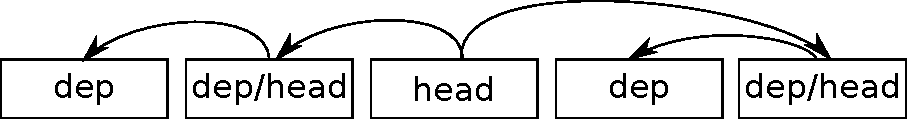
\includegraphics[width=0.9\textwidth]{Figures/SFL-grammar/dependency-dg.pdf}
        \vspace{+22pt}
        \caption{Parent-daughter relations}
        \label{fig:dependency-dg}
    \end{subfigure}%
    \begin{subfigure}{.5\textwidth}
        \centering
        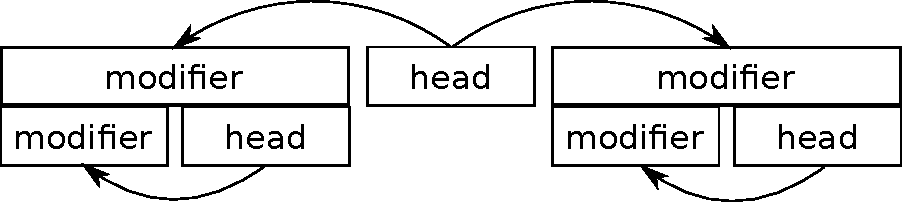
\includegraphics[width=0.9\textwidth]{Figures/SFL-grammar/dependency-sfg.pdf}
        \caption{Sibling head-modifier relations}
        \label{fig:dependency-sfg}
    \end{subfigure}
    \caption{Plain dependency relations in Dependency and Systemic Functional representation}
    \label{fig:dependency-relations}
\end{figure}

Figure \ref{fig:dependency-relations} illustrates side by side the parent-daughter and sibling dependency relations in a simplified form. In Figure \ref{fig:dependency-dg} dependencies are the only relations between the units of structure whereas in Figure \ref{fig:dependency-sfg} are two levels (ranks) of units where the dependency relations are relevant only between sibling elements at the same level within the structure of a unit. As we have seen in Chapter \ref{ch:sfg} knowing only the unit elements is not enough to construct the constituency structure, but it is informative enough for deducing the missing parts. What the Figure \ref{fig:dependency-relations} illustrates is that the two structures resemble each other in a suggestive fashion that will be used below to construct a bridge between descriptions.  

%%%%6. what exactly is the unpacking  principle

The intuitions from the above examples can be laid out by and large in Generalizations \ref{gen:correspondence1}--\ref{gen:correspondence3}. Here I use the term \textit{projection} to refer specifically to the correspondences between theoretical primitives of the two grammars. I say that a primitive in in theory A is projected as another primitive in theory B. The first generalisation is on maximally accounting for the dependency nodes in constituency structure.

\begin{generalization}[Structural Completeness]\label{gen:correspondence1} %maximal accounting
 Each node of the dependency representation is projected, in constituency representation, into one or more units and one or more elements at different rank scales.
\end{generalization}

When translated to a constituency unit, the dependency node, stands for a unit as a whole, the head element of that unit and the word expounding that element. 
For example, the root verb ``seemed'' in a dependency graph corresponds to the clause node and, the Main Verb element and the lexical item which fills the Main Verb of the clause. By analogy, the node ``witness'' stands for the nominal group, the head noun of a Nominal Group and fills the head element of the group.
Even the functional words such as prepositions that in collapsed dependency representation remain orphaned (see Figure \ref{fig:prep-transf2}) have to be accounted in the constituency structure. 

\begin{generalization}[Functional Projection]\label{gen:correspondence2}
    Each dependency relation (alone or contextualised by the word classes of the bridged nodes) is projected into the element of the unit corresponding to the subordinate node. 
\end{generalization}

The dependency relation is primarily responsible for determining the element. For example the ``nsubj'' dependency relation will be projected into a Subject element of a clause unit. Sometimes however, as stated in Generalisation \ref{gen:correspondence2}, the dependency relation alone is not enough and the context given by the governor and subordinate nodes is needed to choose the element. For example the adverbial modifier (advmod) relation alone is not enough to determine into which element to project the subordinate. If the word class context is considered then the verb-to-adverb ``advmod'' relation (VB-advmod-RB) is projected into an Adjunct while the noun-to-adverb ``advmod'' relation (NN-advmod-RB) into is projected Predeictic.  

\begin{generalization}[Substantial Projection]\label{gen:correspondence3}
    Each dependency node projects either the filling or expounding of an element, by a unit of the rank below or by the lexical item of the node. 
\end{generalization}

Generalisation \ref{gen:correspondence3} provides the link between the projected unit with the element of the rank above. For example the subordinate ``witness'' receiving  nominal subject edge from ``seemed'' is responsible for projecting that the Subject element of the clause if filled by the nominal group (headed by the ``witness'' because it is also the governor in the next relation that projects it is the head). The governor ``seemed'', as the root of the tree, is projected into a lexical item which expounds the Main Verb Element (the head of the clause group). In a similar manner, the governor ``witness'' of the determiner (det) relation to ``the'' is projected into a lexical item expounding the Head element (of the nominal group). 

% anotehr example 

\begin{table}[ht]
	\centering
	\begin{tabular}{c|c|c|cc}
        \hline
        \multicolumn{1}{|c|}{\textit{some}}          & \textit{very}   & \textit{small}   & \multicolumn{1}{c|}{\textit{wooden}} & \multicolumn{1}{c|}{\textit{ones}} \\ \hline
        \multicolumn{5}{|c|}{nominal group}                                                                                                                           \\ \hline
        \multicolumn{1}{|c|}{Quantifying Determiner} & \multicolumn{2}{c|}{Epithet}       & \multicolumn{1}{c|}{Classifier}      & \multicolumn{1}{c|}{Head}          \\ \hline
        & \multicolumn{2}{c|}{quality group} &                                      &                                    \\ \cline{2-3}
        & Temperer        & Apex             &                                      &                                    \\ \cline{2-3}
    \end{tabular}
	\caption{SF analysis of Example \ref{ex:small-wooden} (reproduced from Table \ref{tab:example-substructure-analisys-cardiff} )}
	\label{tab:example-substructure-analisys-cardiff-repeated}
\end{table}

\begin{figure}[ht]
	\centering
	\begin{dependency}[dep-style-narrow]
		\begin{deptext}[]
			some/DT \& very/RB \& small/JJ \& wooden/JJ \& ones/NNS \\
		\end{deptext}
		\depedge[edge unit distance =2.2ex]{5}{1}{det}
		\depedge{3}{2}{advmod}
		\depedge{5}{3}{amod}
		\depedge{5}{4}{amod}
	\end{dependency}
	\caption{Dependency analysis for Table \ref{tab:example-substructure-analisys-cardiff-repeated} }
	\label{fig:small-wooden-dependency}
\end{figure}

%The dependency structure is overloaded with two kinds of meaning

Figure \ref{fig:small-wooden-dependency} and Table \ref{tab:example-substructure-analisys-cardiff-repeated} represent the analysis of a nominal group from Example \ref{ex:small-wooden} (``some small very small wooden ones'') in the SFG and the Stanford dependency grammar contrasting the two structures. Consider the dependency relation ``det'' acting as a link between the noun ``ones'' and the determiner ``some''. When translated into the SF variant the dependency relation stands within the nominal group between the Head element (filled by word ``ones'') and the Quantifying Determiner element (filled by the word ``some''). As mentioned earlier all the elements in a unit are equal in the structure so the Head and Quantifying Determiner are siblings. So the items (words) filling those elements are also siblings. How then is the dependency relation established? 

% going again on explaining the SFL dependency

%In SFL there is the concept of Head and Modifier. There is no direct relationship between them, the Modifier and Head stand for two different kinds of meaning and what the Modifier modifies is not the Head per se but the referent denoted by the head (and thus what is construed by the entire unit). It is precisely this modification of the head that is called a (sibling) dependency relation and is seldom mentioned in the SFL literature because it is considered implicit and recoverable from the SF constituency structure.

%strange paragraph, avoid refering to unit anchors
%The Head also is the element that acts as an anchor for the entire unit. In this sense the word ``ones'' realizes not only the Head function (sided with Determiner ``some'') but also anchors the entire unit. The relation between the group and it's elements is one of \textit{componence} (Definition \ref{def:componence}) described in Section \ref{sec:componence}. Yet in the role of unit anchor we cannot say that there is a componence relation between ``one'' and ``some'' because it is merely a proxy to the referent rather than the entire unit. So in this role ``one'' can be said to be standing in a parent-daughter dependency relation to ``some'' incorporating the filling and componence relations.

% example of the relation being unpacked
Lets look at a second example of the two relations ``advmod'' from ``small'' to ``very'' and ``amod'' from ``ones'' to ``small'' in Figure \ref{fig:small-wooden-dependency}. The interesting case here is the item ``small'' which is the head (Apex) of the quality group. I it anchors the meaning of the whole group and the quality group fills the Modifier/Epithet element within the nominal group. What is not covered in previous example is that the Apex ``small'' not only is a representative of the entire group but it also suitable filler on its own for the Modifier element within nominal group. Using the similar translation mechanism as above, this means that, the incoming dependency needs to be unpacked into three levels: the element within the current group (Modifier), the unit class that element is filling (Quality Group) and finally the head of the filler group (Apex). In fact, to be absolutely correct there is one more level. The elements of a unit are expounded by lexical items, so a fourth relation to unpack is the expounding of the Apex by the word ``small''.

%concluding
I just showed how the dependency relation in dependency structure (Figure \ref{fig:dependency-dg}) can be unpacked into compounding elements of a unit (Figure \ref{fig:dependency-sfg}) corresponding to the the sibling dependency considered an indirect relation between the Head and the Modifier (in the Logical metafunction); and then from that using Generalisations \ref{gen:correspondence1}--\ref{gen:correspondence3} deduce the rest of the constituency structure such as the componence relation between unit head and the compounding elements and the filling/expounding relation between the element and the unit right below. 


%do not mention algorithm yet
%TODO[JB] I don't get the impression that we have seen an algorithm yet: just a pointer to the kinds of considerations and differences. So it might help to present a summary which looks more explicitly like an algorithm if you really want to say this here, which would be fine. Do you need to have more information explained before presenting the algorithm? if not, why not put here. If you do, then say very clearly that it will come later, because you don't really mention an algorithm explicitly up to this point. You just say that "the algorithm" will require something... which is not yet very clear.
%In this section I laid the theoretical principle for transforming the dependency structure into systemic functional structure. 

In practice to achieve this level of unpacking two traversals are needed a bottom-up and a top one. This is because the traversal sequence also creates a context that deals with either instantiation a new unit and establishing its elements or with filling an element of a unit above. But more on how to enact the cross theoretical links from this chapter is provided in Section \ref{sec:creation-constituency-graph}.

%TODO [JB] as I mentioned in the previous round of comments, you are going to have to say something more about this. Many many linguists think that null elements are a figment of Chomsky's madness and they are completely unnecessary within a linguistic treatment. So you certainly cannot just assume that they need to be treated. You will have to motivate just why you are going to go this path. You will not be able to prove it is the right path but you should be able to say why it is considered a beneficial or productive kind of solution to your goals in the current thesis.

As motivated elsewhere, I present an account for the unrealised, covert (Null) elements in syntactic structure, using the Governance and Binding Theory. It is also an opportunity to perform a similar cross-theoretical projection exercise.

%
%\todo{close the chapter}
%
%\explain{the problem of bottom up and top down view on the tree structure, due to the fact that head elements plays two roles: of the unit-class(from above) and head-element(from below)}
%\explain{how it is solved with two traversals in the syntactic parsing chapter}
%
%\section{Discussion}
%todo